% Created by tikzDevice version 0.12.3.1 on 2022-09-01 12:21:08
% !TEX encoding = UTF-8 Unicode
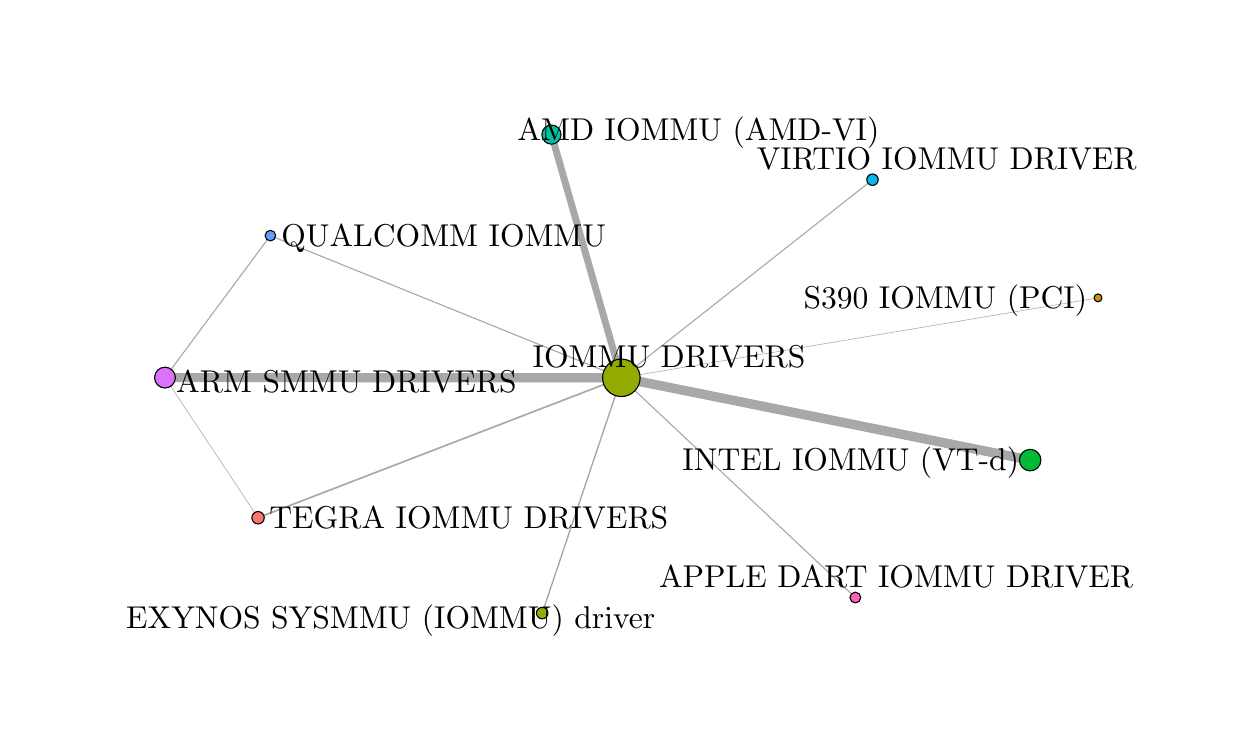
\begin{tikzpicture}[x=1pt,y=1pt]
\definecolor{fillColor}{RGB}{255,255,255}
\path[use as bounding box,fill=fillColor,fill opacity=0.00] (0,0) rectangle (433.62,252.94);
\begin{scope}
\path[clip] (  0.00,  0.00) rectangle (433.62,252.94);
\definecolor{fillColor}{RGB}{255,255,255}

\path[fill=fillColor] (  0.00,  0.00) rectangle (433.62,252.94);
\end{scope}
\begin{scope}
\path[clip] ( 32.75, 32.75) rectangle (403.62,222.94);
\definecolor{drawColor}{gray}{0.66}

\path[draw=drawColor,line width= 2.5pt,line join=round] (189.27,214.30) -- (214.52,126.42);

\path[draw=drawColor,line width= 0.4pt,line join=round] (299.08, 47.01) -- (214.52,126.42);

\path[draw=drawColor,line width= 3.3pt,line join=round] ( 49.61,126.49) -- (214.52,126.42);

\path[draw=drawColor,line width= 0.4pt,line join=round] ( 49.61,126.49) -- ( 87.71,177.79);

\path[draw=drawColor,line width= 0.2pt,line join=round] ( 49.61,126.49) -- ( 83.25, 75.85);

\path[draw=drawColor,line width= 0.5pt,line join=round] (185.92, 41.40) -- (214.52,126.42);

\path[draw=drawColor,line width= 3.4pt,line join=round] (362.24, 96.68) -- (214.52,126.42);

\path[draw=drawColor,line width= 0.4pt,line join=round] (214.52,126.42) -- ( 87.71,177.79);

\path[draw=drawColor,line width= 0.2pt,line join=round] (214.52,126.42) -- (386.76,155.30);

\path[draw=drawColor,line width= 0.6pt,line join=round] (214.52,126.42) -- ( 83.25, 75.85);

\path[draw=drawColor,line width= 0.4pt,line join=round] (214.52,126.42) -- (305.28,198.00);
\definecolor{drawColor}{RGB}{0,0,0}
\definecolor{fillColor}{RGB}{0,193,159}

\path[draw=drawColor,line width= 0.4pt,line join=round,line cap=round,fill=fillColor] (189.27,214.30) circle (  3.46);
\definecolor{fillColor}{RGB}{255,97,195}

\path[draw=drawColor,line width= 0.4pt,line join=round,line cap=round,fill=fillColor] (299.08, 47.01) circle (  1.95);
\definecolor{fillColor}{RGB}{219,114,251}

\path[draw=drawColor,line width= 0.4pt,line join=round,line cap=round,fill=fillColor] ( 49.61,126.49) circle (  3.76);
\definecolor{fillColor}{RGB}{147,170,0}

\path[draw=drawColor,line width= 0.4pt,line join=round,line cap=round,fill=fillColor] (185.92, 41.40) circle (  2.08);
\definecolor{fillColor}{RGB}{0,186,56}

\path[draw=drawColor,line width= 0.4pt,line join=round,line cap=round,fill=fillColor] (362.24, 96.68) circle (  3.89);
\definecolor{fillColor}{RGB}{147,170,0}

\path[draw=drawColor,line width= 0.4pt,line join=round,line cap=round,fill=fillColor] (214.52,126.42) circle (  6.78);
\definecolor{fillColor}{RGB}{97,156,255}

\path[draw=drawColor,line width= 0.4pt,line join=round,line cap=round,fill=fillColor] ( 87.71,177.79) circle (  1.91);
\definecolor{fillColor}{RGB}{211,146,0}

\path[draw=drawColor,line width= 0.4pt,line join=round,line cap=round,fill=fillColor] (386.76,155.30) circle (  1.43);
\definecolor{fillColor}{RGB}{248,118,109}

\path[draw=drawColor,line width= 0.4pt,line join=round,line cap=round,fill=fillColor] ( 83.25, 75.85) circle (  2.24);
\definecolor{fillColor}{RGB}{0,185,227}

\path[draw=drawColor,line width= 0.4pt,line join=round,line cap=round,fill=fillColor] (305.28,198.00) circle (  2.07);

\node[text=drawColor,anchor=base,inner sep=0pt, outer sep=0pt, scale=  1.14] at (242.37,212.10) {AMD IOMMU (AMD-VI)};

\node[text=drawColor,anchor=base,inner sep=0pt, outer sep=0pt, scale=  1.14] at (313.80, 50.65) {APPLE DART IOMMU DRIVER};

\node[text=drawColor,anchor=base,inner sep=0pt, outer sep=0pt, scale=  1.14] at (115.19,121.11) {ARM SMMU DRIVERS};

\node[text=drawColor,anchor=base,inner sep=0pt, outer sep=0pt, scale=  1.14] at (131.16, 35.76) {EXYNOS SYSMMU (IOMMU) driver};

\node[text=drawColor,anchor=base,inner sep=0pt, outer sep=0pt, scale=  1.14] at (297.42, 92.77) {INTEL IOMMU (VT-d)};

\node[text=drawColor,anchor=base,inner sep=0pt, outer sep=0pt, scale=  1.14] at (231.75,130.11) {IOMMU DRIVERS};

\node[text=drawColor,anchor=base,inner sep=0pt, outer sep=0pt, scale=  1.14] at (150.34,173.90) {QUALCOMM IOMMU};

\node[text=drawColor,anchor=base,inner sep=0pt, outer sep=0pt, scale=  1.14] at (331.57,151.38) {S390 IOMMU (PCI)};

\node[text=drawColor,anchor=base,inner sep=0pt, outer sep=0pt, scale=  1.14] at (159.39, 71.93) {TEGRA IOMMU DRIVERS};

\node[text=drawColor,anchor=base,inner sep=0pt, outer sep=0pt, scale=  1.14] at (332.11,201.65) {VIRTIO IOMMU DRIVER};
\end{scope}
\end{tikzpicture}
